\documentclass[a4paper,11pt]{article}
\usepackage[left=2.5cm, right=2.5cm, top=1.5cm, bottom=1.5cm]{geometry}
\usepackage{graphicx}
\usepackage{amssymb}
\usepackage{amsmath}
\usepackage[procnames]{listings}
\usepackage{xcolor}
\usepackage[active,tightpage]{preview}
\usepackage{hyperref}
\usepackage{pythonhighlight}

\hypersetup{ %color attributes of citation, link, etc.
    colorlinks=true,
    linkcolor=blue,
    filecolor=gray,
    urlcolor=blue,
    citecolor=blue,
}

\setlength{\parindent}{0pt}

\renewcommand{\PreviewBorder}{1in}
\newcommand{\Newpage}{\end{preview}\begin{preview}}
\newcommand{\matlab}{\textsc{Matlab}} %very important and totally necessary addition
\newcommand{\parallelsum}{\mathbin{\!/\mkern-5mu/\!}}

\newcommand\Item[1][]{%
  \ifx\relax#1\relax  \item \else \item[#1] \fi
  \abovedisplayskip=0pt\abovedisplayshortskip=0pt~\vspace*{-\baselineskip}}

%'codify' text for snippets
\usepackage{xcolor}
\definecolor{codegray}{gray}{1}
\newcommand{\code}[1]{\colorbox{codegray}{\texttt{#1}}}


\graphicspath{ {../images/} }
           
\begin{document}
\begin{preview}
\title{\LARGE{\textbf{ECEN415 Assignment 1}}}
\author{Niels Clayton : 300437590}
\date{}
\maketitle
\hrule

\section*{Formative}

\begin{enumerate}
    
    \item Sketch Nyquist plots

    \begin{enumerate}
      \item $$ G_1 (s) = \frac{20(s^2+s+0.5)}{s(s+1)(s+10)} $$
      
      \begin{center}
        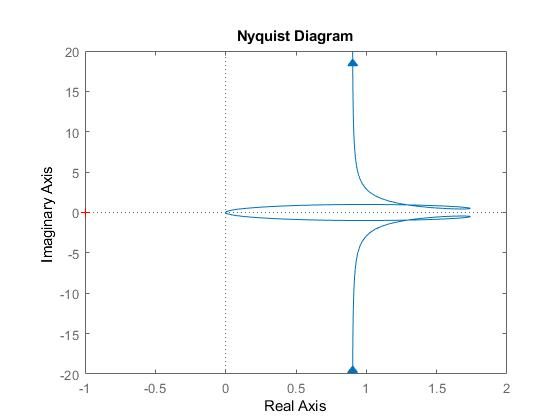
\includegraphics[width=0.7\textwidth]{A_1/1_a.jpg}
      \end{center}

      This system is stable initially, with no right hand poles in the open loop function, and no encirclements of the critical point. Also, since there are no encirclements  that cross the negative real axis, there is no gain that can cause this system to become unstable.\\
      

      \item $$ G_2 (s) = \frac{20(s^2+s+0.5)}{s(s-1)(s+10)} $$

      \begin{center}
        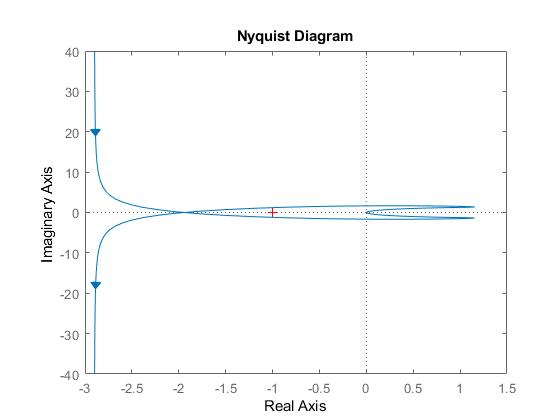
\includegraphics[width=0.7\textwidth]{A_1/1_b.jpg}
      \end{center}

      This system is stable initially, with one right hand poles in the open loop function, and single anticlockwise encirclement of the critical point. However decreasing the gain will cause this encirclement to move away from the critical point, causing the system to become unstable.\\


      \item $$ G_3 (s) = \frac{ s^2+3 }{ (s+1)^2 } $$

      \begin{center}
        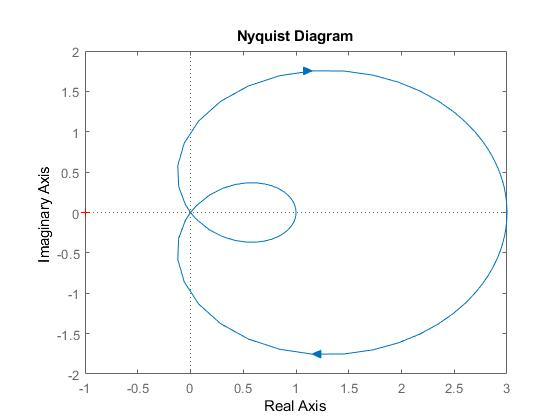
\includegraphics[width=0.7\textwidth]{A_1/1_c.jpg}
      \end{center}

      
      This system is stable initially, with no right hand poles in the open loop function, and no encirclement of the critical point. Also, since there are no encirclements that cross the negative real axis, there is no gain that can cause this system to become unstable.\\

      \item $$ G_4 (s) = \frac{ 3(s+1) }{ s(s-10) } $$

      \begin{center}
        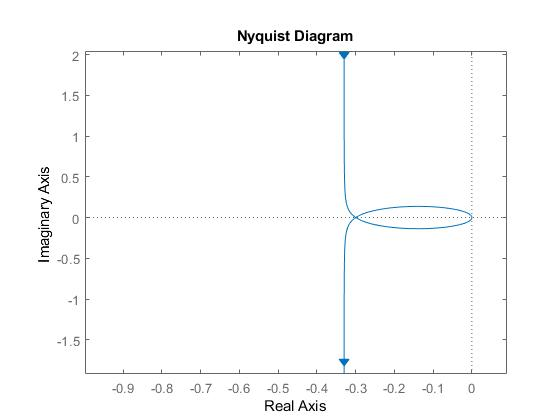
\includegraphics[width=0.7\textwidth]{A_1/1_d.jpg}
      \end{center}

      This system is unstable initially, with one right hand pole in the open loop function, and no encirclement of the critical point. However positive gain will cause the closed loop system to become stable, adding an anticlockwise encirclement of the critical point.\\
    \end{enumerate}


\hrule

\item Affects of delay on a closed loop system.

\begin{enumerate}
  
  \item $ G(s) = \frac{4}{s+2} $ With a delay of 0.2s
  
  \begin{center}
    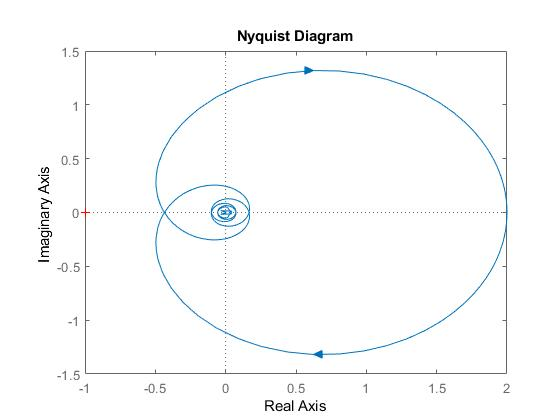
\includegraphics[width=0.7\textwidth]{A_1/2_a_nyquist.jpg}
  \end{center}

  This system is stable initially, with no right hand poles in the open loop function, and no encirclement of the critical point. However by increasing the gain of this system we can cause a clockwise encirclement of the critical point. This will place a pole in the right hand plain of the closed loop system, and cause it to become unstable. 

  To find the gain at which this occurs we look at the location that the encirclement crosses the negative real axis, we can find this value to be -0.435. From here we find the gain that causes this point to be greater than the critical point. 

  $$ \mathrm{Gain} = \frac{-1}{-0/435} = 2.294$$\\


  \item Step response of $G(s)$ at a gain of 1, and a gain of 2.294

  \begin{center}
    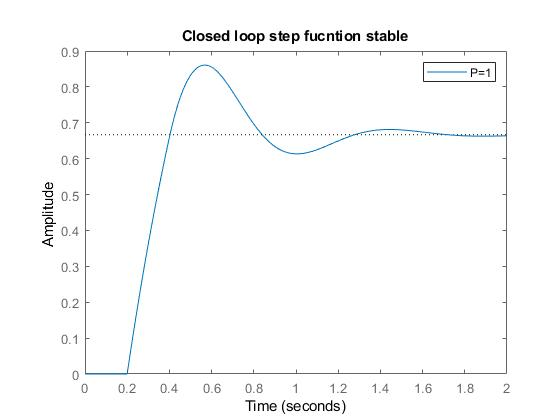
\includegraphics[width=0.7\textwidth]{A_1/2_b_stable.jpg}
  \end{center}

  Step response of  $G(s)$ at a gain of 1.

  \begin{center}
    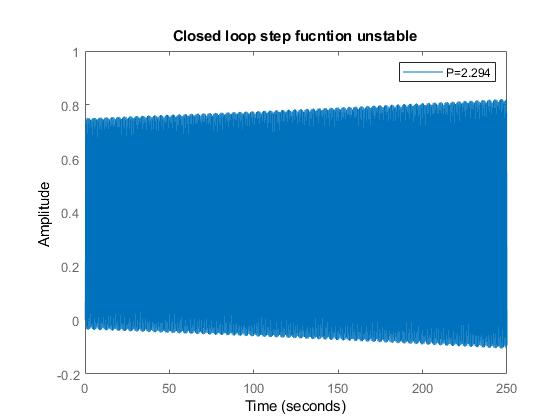
\includegraphics[width=0.7\textwidth]{A_1/2_b_unstable.jpg}
  \end{center}
  
  Step response of $G(s)$ at a gain of 2.294.\\

  This system behaves as was predicted by the Nyquist plot.\\\\

  \item Through guess and check it was found that a delay of 0.61 seconds caused the system to become unstable. This can be seen in both the Nyquist plot and step response of the closed loop system.
  
  \begin{center}
    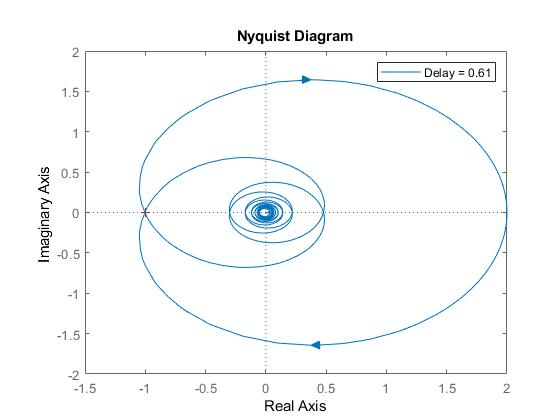
\includegraphics[width=0.7\textwidth]{A_1/2_c_nyquist.jpg}
  \end{center}

  \begin{center}
    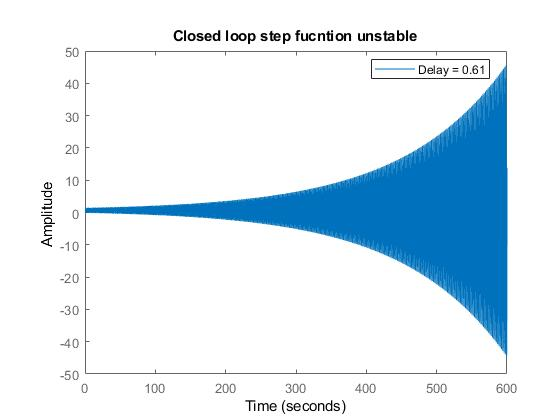
\includegraphics[width=0.7\textwidth]{A_1/2_c_unstable.jpg}
  \end{center}

\end{enumerate}

\hrule
  
\item Compare the different z-domain transfers of $G(s) = \frac{1000}{s+1000}$\\

For this we will be comparing the step response, impulse response, and bode plots for a range of differing methods of converting from continuous time to discrete time. We will be looking at the bilinear and bilinear with pre-warp conversion, impulse invariance conversion, and the matched pole zero conversion.\\\\

Each of these conversions has it's pros and cons, bilinear and bilinear with pre-warp conversions will preserve the stability of the original system, however this conversion suffers from inaccuracy at higher frequencies. The impulse invariance conversion preserves the impulse response of the continuous time system, however can vary greatly for the step response and does not guarantee the preservation of stability. Finally the matched pole zero conversion preserves the location of all poles in zeros within the z-plane.\\\\

In the following images we can see these conversions plotted against each other.

\begin{center}
  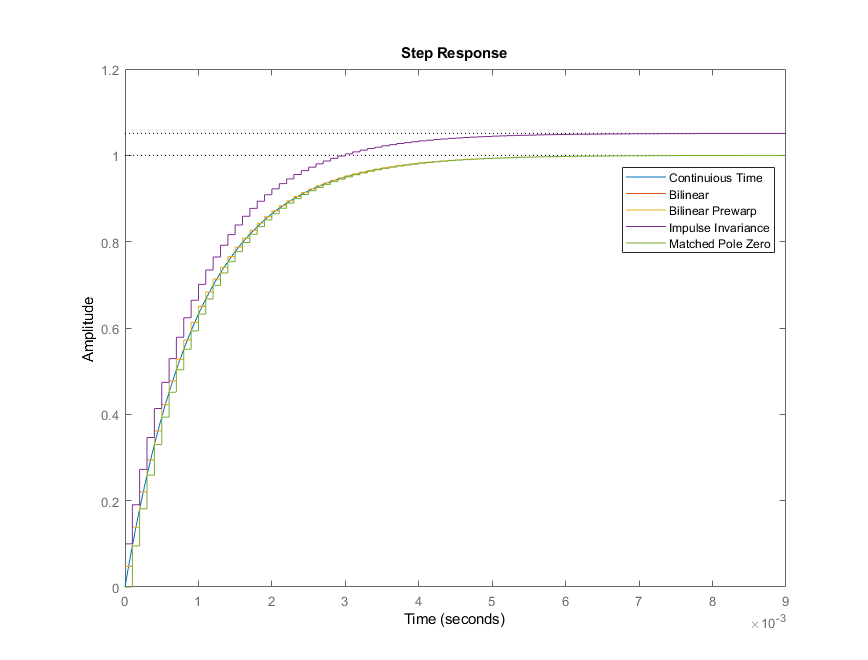
\includegraphics[width=0.9\textwidth]{A_1/3_step.png}
\end{center}

When comparing the step responses of these conversions we can clearly see that the impulse invariance conversion method does not preserve the steady state gain of the system. All other conversion methods however seem to produce a close approximation of the continuous time system.

\begin{center}
  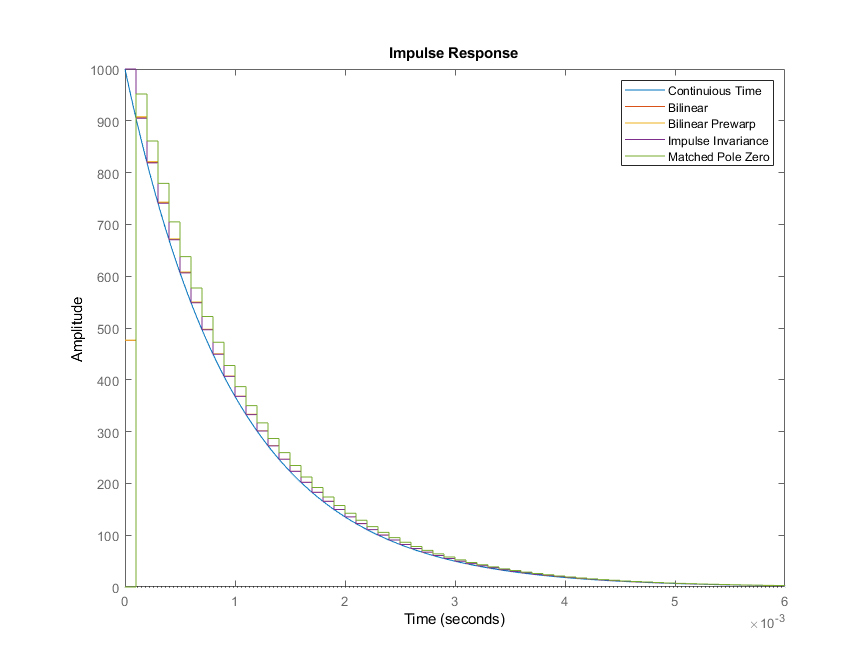
\includegraphics[width=0.9\textwidth]{A_1/3_impulse.png}
\end{center}

When comparing the impulse responses we can see that the impulse invariance conversion method matches exactly the impulse response of the continuous time system. We can also see that the matched pole zero conversion does not preserve the impulse response, with a noticeable time delay compared to the others. 

\begin{center}
  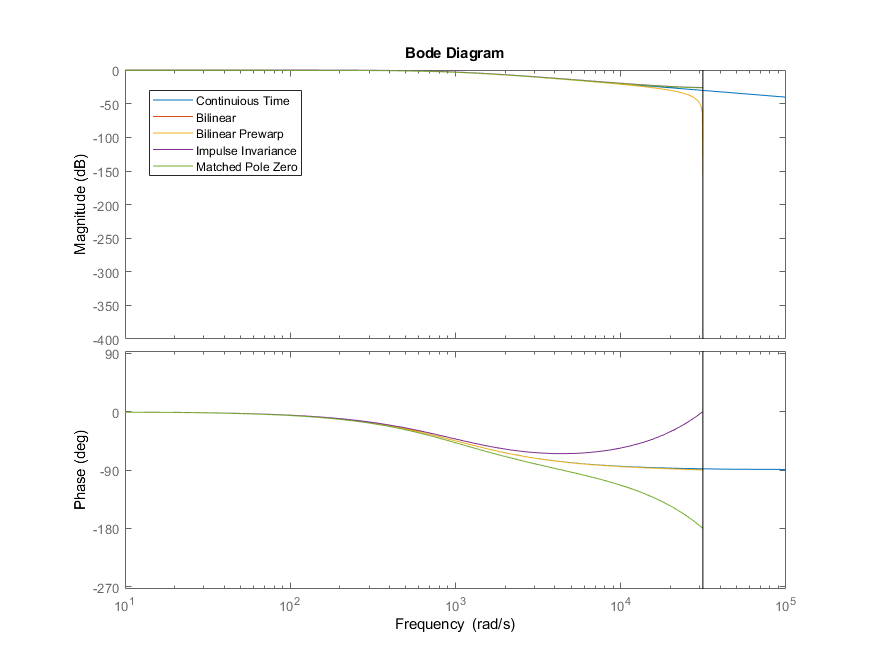
\includegraphics[width=0.9\textwidth]{A_1/3_bode.png}
\end{center}

When looking at the bode plots, we can see that both the bilinear and bilinear with pre-warp conversions match the magnitude and phase plots the best. We can also clearly see that both the matched pole zero and impulse invariance conversions greatly affect the phase response at higher frequencies. \\

\hrule
\end{enumerate}

\section*{Summative}

\begin{enumerate}

  \item

  \begin{enumerate}

  \item At what angular frequency does $D(s) = e^{st_d}$ cause a -90$^o$ phase shift:\\\\

  Using $s = \sigma + j\omega$
  \begin{align*}
    D(s) = e^{st_d} &\rightarrow e^{(\sigma + j\omega)t_d}\\
    &= e^{\sigma t_d} \cdot e^{j\omega t_d}\\
    &= e^{\sigma t_d} \cdot \cos(\omega t_d) + j \sin(\omega t_d)\\ 
  \end{align*}

  This is a complex number in polar form, where $j \sin(\omega t_d)$ refers to the phase of the complex number. From this we can associate the phase of $D(s)$ to $\omega$.

  \begin{align*}
    \angle D(s) &= \omega t_d\\\\
    \omega &= \frac{\angle D(s)}{t_d}
  \end{align*}

  From here we have a function for frequency when $\angle D(s) = -90 = \frac{\pi}{2}$

  $$ \omega = \frac{\pi}{2 t_d} $$

  \item 

  Unity gain: 1000 rads$^{-1}$\\
  Phase shift of $\frac{-\pi}{12}$ or -15$^o$\\
  $$ \omega = \frac{\angle D(s)}{t_d}$$ 
  $$ t_d = \frac{\angle D(s)}{\omega} = \frac{-\pi}{12\cdot1000} = \frac{-\pi}{12000}$$\\
  $$ t_d = 261 \mu s$$\\

  \item 

  Using the \code{pade()} function within matlab, we take the first order and second order Pad\`{e} approximations of the pure delay. Then through elimination I have found the delay that provides a phase of -15$^o$ at the unity gain frequency of 1000 rads$^{-1}$.\\\\

  Using the first order Pad\`{e} approximation of a delay we can allow for a $270 \mu s$ delay before the system becomes unstable.
  \begin{center}
    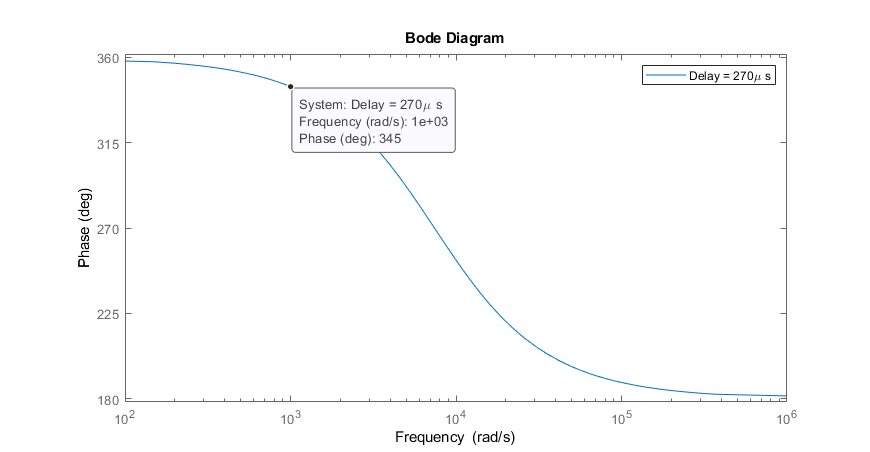
\includegraphics[width=0.9\textwidth]{Summative/first_order_pade.png}
  \end{center}

  Using the second order Pad\`{e} approximation of a delay we can allow for a $261 \mu s$ delay before the system becomes unstable, which is the same as a pure delay.
  \begin{center}
    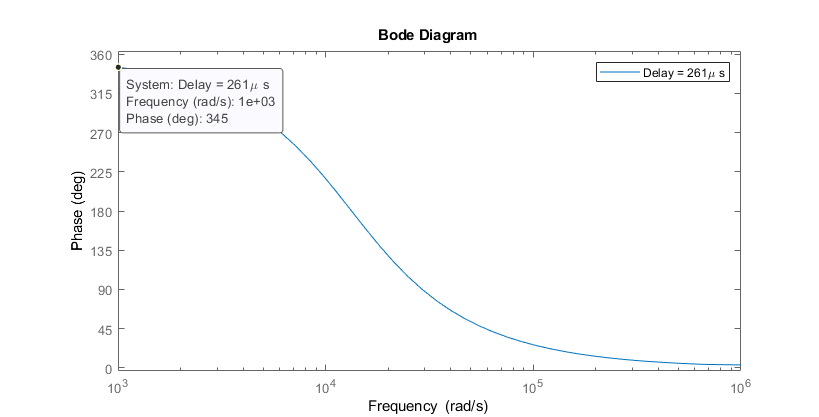
\includegraphics[width=0.9\textwidth]{Summative/second_order_pade.png}
  \end{center}

\end{enumerate}

\hrule 

\item

The system $G(s) = \frac{15}{(s+1)(s+2)}$ is to be used in a sampled data system.

By looking at the root locus plot of $G(s)$ we can see that this system has two poles in the right half plane, and that there is no gain that can cause the system to become unstable. 

\begin{center}
  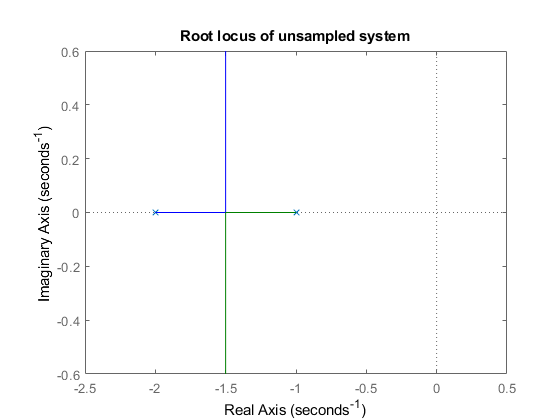
\includegraphics[width=0.9\textwidth]{Summative/rlocus_unsampled.png}
\end{center}

To sample this system we will use the Pad\`{e} approximation of the ideal zero order hold transfer function:

\begin{align*}
  \frac{1-e^{s t_s}}{s} &\approx\frac{1}{s}\frac{1-\frac{s t_s}{2}}{1+\frac{s t_s}{2}}\\
  &= \frac{2}{s+\frac{2}{t_s}}
\end{align*}

By using this transfer function to sample $G(s)$, we can clearly see that it introduces a third pole to the right hand plane at $\frac{2}{t_s}$. by adding this third pole, the departure angles for the two original poles changes to $\frac{180}{P-Z} = \frac{180}{3} = 60^\circ$. This means that after sampling there now exists a gain for which the system will become unstable, this is shown in the image below. 

\begin{center}
  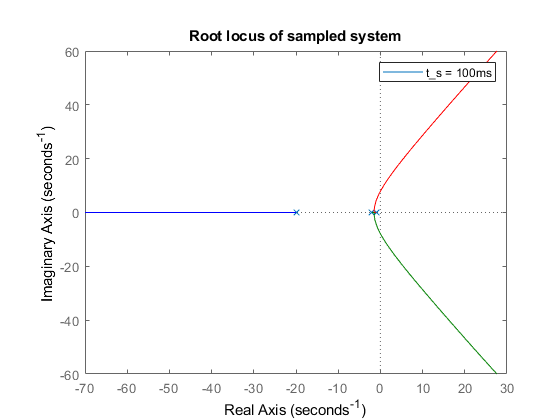
\includegraphics[width=0.9\textwidth]{Summative/rlocus_sampled_100ms.png}
\end{center}

We can also tell from the transfer function of the sampler that for smaller sampling frequencies the additional pole moves further from 0, and becomes less dominant.\\\\

By looking at the bode plot of the unsampled system we can find the unity gain of the system to be at a frequency of 3.55 rads$^{-1}$, or 0.565$H$z.

\begin{center}
  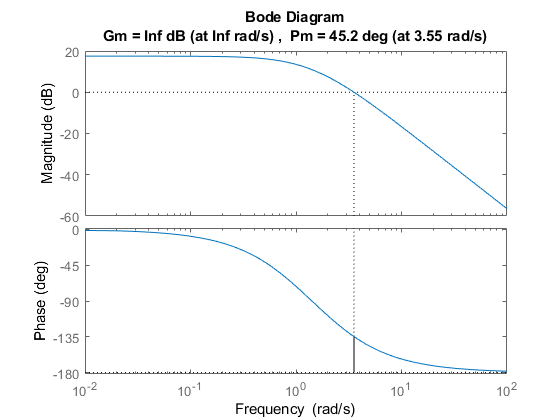
\includegraphics[width=0.9\textwidth]{Summative/bode_unsampled.png}
\end{center}

When sampling at unity gain of the system (5.65$H$z), we can see that the gain margin is 24.3 dB.

\begin{center}
  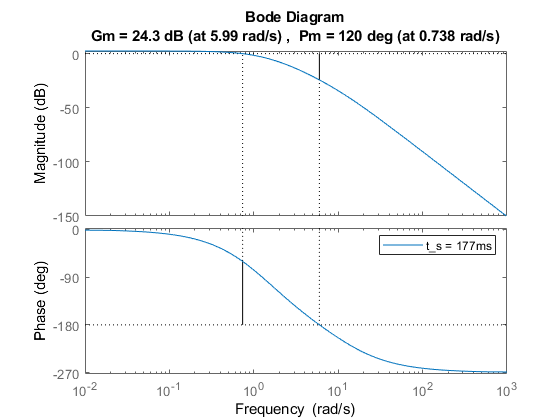
\includegraphics[width=0.9\textwidth]{Summative/bode_sampled_177ms.png}
\end{center}

\hrule


\item Given a system with a phase margin of 10$^\circ$ and 10 kHz unity gain frequency, we must design a second order Butterworth filter that is capable of attenuating aliased signals by at least 40 dB. We must also design this system such that this filter can be sampled at least ten times the unity gain frequency without causing instability.\\\\

The transfer function of the Butterworth second order filter is:
$$ G_b (s) = \frac{\omega_c^2}{s^2 + \sqrt{2}\omega_c s + \omega_c^2} \;\;\;\; \mathrm{Where \;} \omega_c \mathrm{\; is \; the \; corner \; frequency}$$ 

Using these constraints we can relate $\omega_c$ to the sampling frequency $f_s$, as we know the corner frequency must be a decade below half of the sampling frequency to properly attenuate the aliasing.
$$ \omega_c = f_s /2 / 10 = \frac{f_s}{20}$$

Using matlab to iterate through frequencies beginning at the minimum 100 kHz sampling frequency, we apply a zero order hold sampler to the generated Butterworth filter. By looking at the phase of the filter at the systems unity gain frequency of 10 kHz, we check if the the phase is less than 10$^\circ$, indicating that the filter will be within the required phase margin. This process was done using both the Pad\`{e} approximation of the zero order hold sampler and the ideal sampler, both of which can be seen below. \\\\


Sampled using the Pad\`{e} approximation of the zero order hold sampler. Sampling frequency of 1807120 Hz.
\begin{center}
  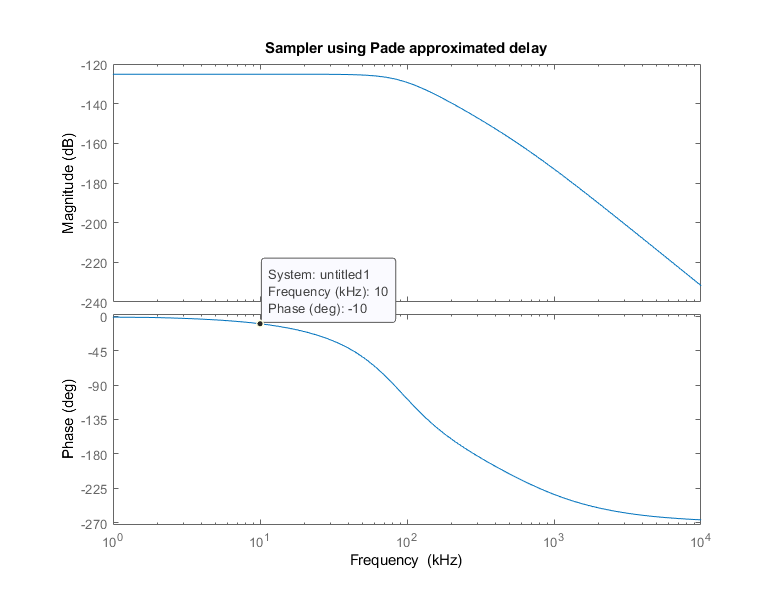
\includegraphics[width=0.9\textwidth]{Summative/butterworth_sample_pade.png}
\end{center}

Sampled using the ideal zero order hold sampler. Sampling frequency of 1807138 Hz.
\begin{center}
  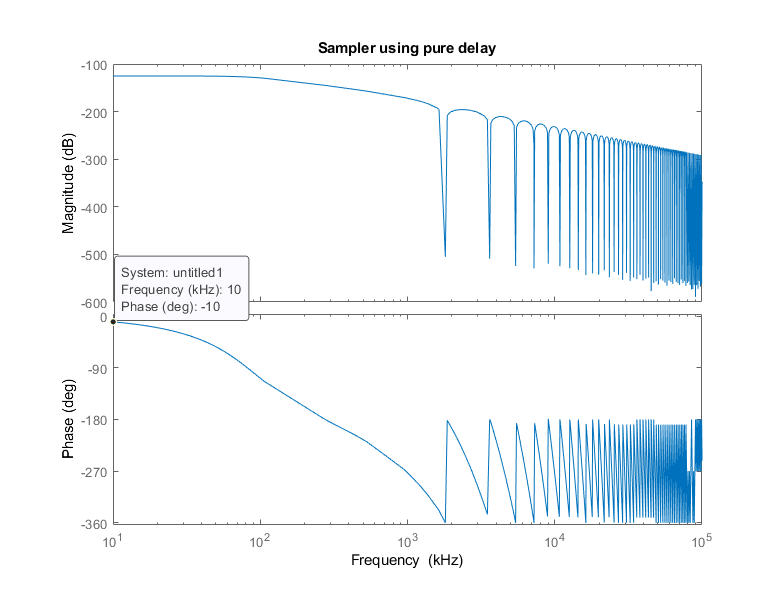
\includegraphics[width=0.9\textwidth]{Summative/butterworth_sample.png}
\end{center}

On both of these plots it can be seen that a phase of -10 $^\circ$ was achieved at the systems unity gain frequency. It can also be seen that both the  Pad\`{e} and idea sampled provide very similar results.\\\\

Overall, if a sampling frequency over 1807138 Hz is chosen, we know that that the antialiasing filter's phase shift will bot exceed the allowable phase margin of the system.  \\

\end{enumerate}

\section*{Matlab Code}

\subsection*{Formative}
  \hrule  
  \lstinputlisting{../Assignment_1_Formative.m}
  \hrule 

\subsection*{\\\\Summative}
\hrule 
\lstinputlisting{../Assignment_1_Summative.m}
\hrule 

\end{preview}
\end{document}